\documentclass[letterpaper,9pt]{article}

\usepackage{latexsym}
\usepackage[empty]{fullpage}
\usepackage{titlesec}
\usepackage{marvosym}
\usepackage[usenames,dvipsnames]{color}
\usepackage{verbatim}
\usepackage{enumitem}
\usepackage[hidelinks]{hyperref}
\usepackage{fancyhdr}
\usepackage[english]{babel}
\usepackage{tabularx}
\usepackage[absolute,overlay]{textpos} % Added package for positioning
\usepackage{graphicx} % Added package for including images
\input{glyphtounicode}

%----------FONT OPTIONS----------
% sans-serif
% \usepackage[sfdefault]{FiraSans}
% \usepackage[sfdefault]{roboto}
% \usepackage[sfdefault]{noto-sans}
% \usepackage[default]{sourcesanspro}

% serif
% \usepackage{CormorantGaramond}
% \usepackage{charter}

\pagestyle{fancy}
\fancyhf{} % clear all header and footer fields
\fancyfoot{}
\renewcommand{\headrulewidth}{0pt}
\renewcommand{\footrulewidth}{0pt}

% Adjust margins
\addtolength{\oddsidemargin}{-0.5in}
\addtolength{\evensidemargin}{-0.5in}
\addtolength{\textwidth}{1in}
\addtolength{\topmargin}{-.5in}
\addtolength{\textheight}{1.0in}

\urlstyle{same}

\raggedbottom
\raggedright
\setlength{\tabcolsep}{0in}

% Sections formatting
\titleformat{\section}{
  \vspace{-4pt}\scshape\raggedright\large
}{}{0em}{}[\color{black}\titlerule \vspace{-5pt}]

% Ensure that generate pdf is machine readable/ATS parsable
\pdfgentounicode=1

%-------------------------
% Custom commands
\newcommand{\resumeItem}[1]{
  \item\small{
    {#1 \vspace{-2pt}}
  }
}

\newcommand{\resumeSubheading}[4]{
  \vspace{-2pt}\item
    \begin{tabular*}{0.97\textwidth}[t]{l@{\extracolsep{\fill}}r}
      \textbf{#1} & #2 \\
      \textit{\small#3} & \textit{\small #4} \\
    \end{tabular*}\vspace{-7pt}
}

\newcommand{\resumeSubSubheading}[2]{
    \item
    \begin{tabular*}{0.97\textwidth}{l@{\extracolsep{\fill}}r}
      \textit{\small#1} & \textit{\small #2} \\
    \end{tabular*}\vspace{-7pt}
}

\newcommand{\resumeProjectHeading}[2]{
    \item
    \begin{tabular*}{0.97\textwidth}{l@{\extracolsep{\fill}}r}
      \small#1 & #2 \\
    \end{tabular*}\vspace{-7pt}
}

\newcommand{\resumeSubItem}[1]{\resumeItem{#1}\vspace{-4pt}}

\renewcommand\labelitemii{$\vcenter{\hbox{\tiny$\bullet$}}$}

\newcommand{\resumeSubHeadingListStart}{\begin{itemize}[leftmargin=0.15in, label={}]}
\newcommand{\resumeSubHeadingListEnd}{\end{itemize}}
\newcommand{\resumeItemListStart}{\begin{itemize}}
\newcommand{\resumeItemListEnd}{\end{itemize}\vspace{-5pt}}

%-------------------------------------------
%%%%%%  RESUME STARTS HERE  %%%%%%%%%%%%%%%%%%%%%%%%%%%%

\begin{document}

% Add this code to include the photograph
\begin{textblock*}{2cm}(18cm,0.5cm) % Adjust position and size as needed
  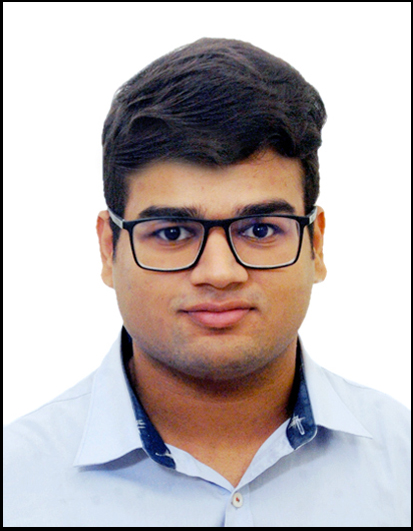
\includegraphics[width=2cm,height=2.5cm,keepaspectratio]{photo.jpg}
\end{textblock*}

%----------HEADING----------
\begin{center}
    \textbf{\Huge \scshape Devansh Rastogi} \\ \vspace{10pt}
    \small \href{mailto:dvcam.rastogi1980@gmail.com}{\underline{devansh.rastogi6877@gmail.com}} $|$ 
    \href{https://linkedin.com/in/rastogidevansh}{\underline{linkedin.com/in/rastogidevansh}} $|$
    \href{https://github.com/primeDevansh}{\underline{github.com/primeDevansh}}
\end{center}

%-----------EDUCATION-----------
\section{Education}
  \resumeSubHeadingListStart
    \resumeSubheading
      {Indian Institute of Technology Madras}{Chennai, Tamil Nadu}
      {Bachelor of Science in Data Science and Applications}{Jan. 2024 -- Dec. 2027}
    \resumeSubheading
      {Guru Gobind Singh Indraprastha University}{Dwarka, Delhi}
      {Bachelor of Technology in Computer Science, Minor in AI \& ML}{Sep. 2021 -- July 2025}
  \resumeSubHeadingListEnd

%-----------EXPERIENCE-----------
\section{Experience}
  \resumeSubHeadingListStart
    \resumeSubheading
      {Research Intern}{May 2024 -- Present}
      {IIIT-Delhi}{On-site, Networked Systems Lab}
      \resumeItemListStart
      % You have to describe your ROLE here!
        \resumeItem{Collaborated with a team in the Networked Systems (NetSys) Lab on a project associated with Marvell Technologies and IIT Hyderabad, focusing on simulating network traffic patterns for LLM inferencing workloads}
        \resumeItem{Conducted in-depth research on RDMA technology and designed a virtual RDMA communication infrastructure for efficient VM-to-VM communication}
        % \resumeItem{Designed a virtual RDMA communication infrastructure for efficient VM-to-VM communication}
        \resumeItem{Acquired extensive knowledge of operating system fundamentals and low-level C programming concepts}
      \resumeItemListEnd

    \resumeSubheading
      {Data Science Intern}{Feb. 2024 -- Mar. 2024}
      {IBM SkillsBuild | CSRBOX}{Remote}
      \resumeItemListStart
        \resumeItem{Acquired sound technical knowledge of data cleaning and preparation, statistical analysis and data visualization}
        \resumeItem{Tested this knowledge on the analysis of a real-world project through a case-study}
        \resumeItem{Learned to interpret the results of the analysis and presented them effectively}
      \resumeItemListEnd

    \resumeSubheading
      {Liaison Officer}{July 2023}
      {G20 Conference on Crime and Security in the age of NFTs, AI \& Metaverse}{Gurugram, Haryana}
      \resumeItemListStart
        \resumeItem{Facilitated collaboration among G20 nations' representatives}
        \resumeItem{Ensured seamless communication on emerging NFT, AI, and Metaverse challenges}
        \resumeItem{Fostered collective strategies for global crime and security}
    \resumeItemListEnd

  \resumeSubHeadingListEnd

%-----------PROJECTS-----------
\section{Projects}
    \resumeSubHeadingListStart
    
    \resumeProjectHeading
          {\textbf{RDMA Traffic Generator for Distributed LLM Inferencing Workload} $|$ \emph{PyTorch, TorchRun}}{June 2024 -- Present}
          \resumeItemListStart
            \resumeItem{Collaborated with a team to understand network packet traces in a distributed-computing environment for LLM inferencing workload}
            \resumeItem{Set up a an RDMA communication infrastructure for 2 rack servers to communicate with each other for a distributed-computing environment}
            \resumeItem{Generated RDMA traffic for ditributed LLM inferencing workload using PyTorch's TorchRun library}
          \resumeItemListEnd

    \resumeProjectHeading
			{\textbf{Hotel Reservation System} $|$ \emph{Ballerina, Choreo, React.js}}{Feb. 2024}
          \resumeItemListStart
            \resumeItem{Implemented an API service using Ballerina programming language to demo a simple hotel reservation use case}
            \resumeItem{Developed front-end using React.js and built this project as a part of a buildathon conducted at my college}
            \resumeItem{Acquired sound technical knowledge about Ballerina and Choreo concepts}
            \resumeItem{Deployed the fully working Ballerina application on Azure cloud using Choreo}
          \resumeItemListEnd

    \resumeProjectHeading
          {\textbf{Classify Song Genres from Audio Data} $|$ \emph{Python, NumPy}}{Jan. 2024 -- Feb. 2024}
          \resumeItemListStart
            \resumeItem{Applied machine learning algorithms to classify songs into genres}
            \resumeItem{Prepared the data set to apply principal component analysis (PCA)}
            \resumeItem{Trained a decision tree to classify the genre}
            \resumeItem{Used cross-validation to evaluate the models}
          \resumeItemListEnd

    \resumeSubHeadingListEnd

%-----------PROGRAMMING SKILLS-----------
\section{Technical Skills}
 \begin{itemize}[leftmargin=0.15in, label={}]
    \small{\item{
     \textbf{Languages}{: Python, C, C++, Swift, SQL} \\
    %  You can add MPI for parallel computing.
     \textbf{Frameworks}{: Libfabric, SwiftUI} \\
     \textbf{Developer Tools}{: Git/GitHub, VS Code, Xcode, JupyterLab, RStudio} \\
     \textbf{Hardware Skills}{: Arduino, Raspberry-Pi, Circuit Design, Sensor Integration, GPIO Programming} \\
}}
\end{itemize}

%----------EXTRA-CURRICULAR ACTIVITIES------
\section{Extra-Curricular Activities}
 \begin{itemize}[leftmargin=0.15in, label={}]
    \small{\item{
     \textbf{Sports:}{ Engaged in active participation and proficient organization of basketball and cricket events} \\
     \textbf{YouTube:}{ Passionate YouTube content creator with 100+ subscribers, featuring technical and diverse content} \\
     \textbf{Volunteering:}{ Engaged in regular, independent volunteering activities involving the preparation and distribution of freshly cooked meals to individuals in need}
    }}
 \end{itemize}

%-------------------------------------------
\end{document}
